% !TeX root = surprises.tex

\selectlanguage{hebrew}

\chapter{פתרון משוואות ריבועיות}\label{c.quadratic}

\L{Poh-Shen Loh}
הציע שיטת למצוא פרתונות למשואות ריבועית המבוססת על היחס בין הקדמים של הפולינום הריבועי לבין שורשיו. סעיף% 
~\ref{s.traditional}
סוקר את השיטות הרגילות למצוא פתרונות למשוואות ריבועיות וסעיף%
~\ref{s.computing}
מנסה לשכנע את הקורא שהשיטה של
\L{Loh}
הגיונית ואז מסביר איך לחשב את השורשים. בסעיף%
~\ref{s.examples}
נדגים את החישוב עבור שני פולינומים ריבועיים וחישוב דומה עבור פולינום ממעלה רביעית. סעיף%
~\ref{s.general}
מפתח את הנוסחה הרגילה לחישוב שורשים מהנוסאות של 
\L{Loh}.

אלגברה והסימונים האלגבריים הם פיתוח יחסית חדשה. תקופות קדומות יותר, מתמטיקאים השתמשו כמעט אך ורק בגיאומטריה, ולכן מעניין לעיין בבניות הגיאומטריות של
\L{al-Khwarizmi}
עבור הנוסחאות במשוואות ריבועיות (סעיף%
~\ref{s.khwar}).
סעיף%
~\ref{s.cardano}
מציג בנייה של ש-%
\L{Cardano}
השתמש בה בפיתוח הנוסחאות עבור השורשים למשוואה קובית.

סעיף%
~\ref{s.lill-quadratic}
מציג שיטות אחרות למצוא את השורשים של משוואות ריבועיות.%
\footnote{קריאת פרק%
~\ref{c.origami-cube}
היא דרישת קדם להבנה מליאה של השיטות הללו.}
סעיף%
~\ref{s.numerical}
דן בחישוב נומרי של השורשים של משוואות ריבועיות.

\section{השיטות המסורתיות לפתרון משוואות ריבועיות}\label{s.traditional}

כל תלמיד לומד את הנוסחה למצוא את השורשים של משוואה ריבועית
$ax^2+bx+c=0$:
\[
x_1, x_2 = \frac{-b\pm\sqrt{b^2-4ac}}{2a}\,.
\]
נגביל את עצמנו למשוואות שהמקדם הראשון הוא אחד, כי תמיד אפשר לחלק ב-%
$a$.
השורשים של
$x^2+bx+c=0$
הם:
\begin{equation}\label{eq.quadratic-roots}
x_1, x_2 = \frac{-b\pm\sqrt{b^2-4c}}{2}\,.
\end{equation}
שיטה נוספת למציאת שורשים של משוואות ריבועיות היא לפרק את הפולינום הריבועי. לעתים קל לפרק את הפולינום:

\begin{equation}\label{eq.quadratic-lill}
x^2-4x+3= (x-1)(x-3)=0\,.
\end{equation}
קשה הרבה יותר לפרק את הפולינום:
\[
x^2-2x-24= (x-r_1)(x-r_2)=0\,,
\]
כי יש לבדוק מספר רב של זוזות שורשים האפשריים:
\[
(\pm 1,\mp 24)\,, (\pm 2,\mp 12)\,, (\pm 3,\mp 8)\,, (\pm 4,\mp 6)\,.
\]

%%%%%%%%%%%%%%%%%%%%%%%%%%%%%%%%%%%%%%%%%%%%%%%%%%%%%%%

\section{הקשר בין המקדמים לשורשים}\label{s.computing}


\begin{theorem}\label{thm.roots-coefficients}
אם
$r_1,r_2$
הם השורשים של
$x^2+bx+c$
אזי:
\[
(x-r_1)(x-r_2)=x^2 - (r_1+r_2)x + r_1r_2=x^2+bx+c\,,
\]
ולכן גם אם ערכם של השורשים לא ידועים, כן ידוע ש:
\begin{equation}\label{eq.viete-quad}
r_1+r_2 = -b\,,\quad\quad r_1r_2=c\,.
\end{equation}
\end{theorem}
למעשה אין מה להוכיח כי התוצאה מתקבלת מהחישוב.

נסתכל על מספר ערכים עבור
$-b,r_1,r_2$
ונסמן ב-%
$m_{12}$
את הממוצע של
$r_1,r_2$:
\[
\renewcommand{\arraystretch}{1.3}
\begin{array}{|r|r|r|r|}
\hline
-b& r_1 & r_2 &m_{12}\\\hline
\hline
33 & 12 & 21 & 16\frac{1}{2}\\\hline
33 & 8 & 25 & 16\frac{1}{2}\\\hline
33 & 1 & 32 & 16\frac{1}{2}\\\hline
\hline
-4 & -16 & 12 & -2 \\\hline
-4 & -4 & 0 & -2 \\\hline
-4 & -3 & -1 & -2 \\\hline
\end{array}
\]
עבור כל משוואה ריבועית, הממוצע של שני השורשים קבוע:
\[
m_{1,2}=\frac{r_1+r_2}{2}=
\frac{(-b-r_2)+r_2}{2}=
\frac{-b}{2}+\frac{-r_2+r_2}{2}=
-\frac{b}{2}\,.
\]
יהי 
$s$ 
מספר כלשהו, אזי:
\[
-b=-b+s+(-s)=\left(\frac{-b}{2}+s\right) + \left(\frac{-b}{2}-s\right)=r_1+r_2\,.
\]
אם שורש אחד נמצא במרחק
$s$
מהממוצע, השורש השני נמצא במרחק
$-s$
מהממוצע:
\[
\renewcommand{\arraystretch}{1.3}
\begin{array}{|r|r|r|r|r|r|}
\hline
-b& r_1 & r_2 & m_{12}& m_{12}-r_1 & m_{12}-r_2\\\hline\hline
33 & 12 & 21 & 16\frac{1}{2}&4\frac{1}{2} & -4\frac{1}{2}  \\\hline
33 & 8 & 25 & 16\frac{1}{2}&8\frac{1}{2}&-8\frac{1}{2}\\\hline
33 & 1 & 32 & 16\frac{1}{2}&15\frac{1}{2}&-15\frac{1}{2}\\\hline
\hline
-4 & -16 & 12 & -2 &14& -14\\\hline
-4 & -4 & 0 & -2&2&-2 \\\hline
-4 & -3 & -1 & -2&1&-1 \\\hline
\end{array}
\]
איור%
~\ref{f.loh-roots1}
מראה את היחסים הללו עבור
$r_1,r_2=2,6$,
כאשר
$m_{12}=4, s=2$:
\begin{figure}[htb]
\begin{center}
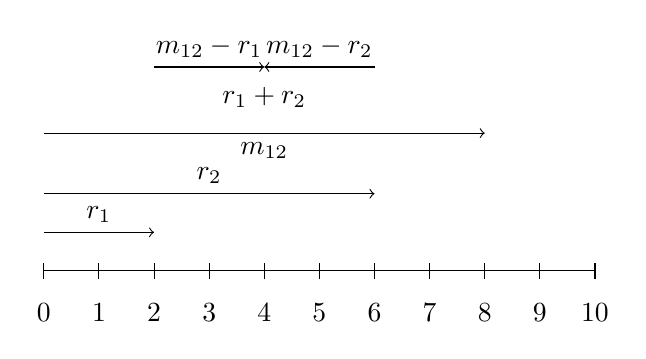
\begin{tikzpicture}[scale=.7]
\begin{scope}[yshift=-4mm]
\draw (0,0) -- (10,0);
\foreach \x in {0,1,...,10}
  \draw (\x,-1.5mm) -- +(0,3mm) node[below,yshift=-4mm] {$\x$};
\draw[->,yshift=7mm] (0,0) -- node[above] {$r_1$} (20mm,0);
\draw[->,yshift=14mm] (0,0) -- node[above] {$r_2$} (60mm,0);
\end{scope}
\draw[->,yshift=21mm] (0,0) -- node[above,yshift=2mm] {$r_1+r_2$} (80mm,0);
\coordinate (M) at (40mm,21mm);
\vertex{M};
\node[below] at (40mm,21mm) {$m_{12}$};
\begin{scope}[yshift=3mm]
\draw[->,yshift=30mm] (20mm,0mm) -- node[above] {$m_{12}-r_1$} +(20mm,0);
\draw[->,yshift=30mm] (60mm,0mm) -- node[above] {$m_{12}-r_2$} +(-20mm,0);
\end{scope}
\end{tikzpicture}
\end{center}
\caption{היחס בין 
$r_1,r_2=2,6$
והממוצע שלהם
$m_{12}=4$}
\label{f.loh-roots1}
\end{figure}
אם נבחר ערכים אחרים
$r_1,r_2=3,5$
עבורם
$r_1+r_2=8$, $m_{12}=4$ 
נשאר ללא שינוי, אבל
$s=1$
משתנה (איור%
~\ref{f.loh-roots2}).
\begin{figure}[htb]
\begin{center}
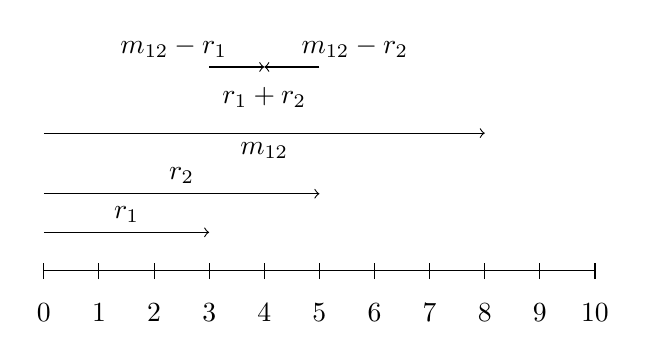
\begin{tikzpicture}[scale=.7]
\begin{scope}[yshift=-4mm]
\draw (0,0) -- (10,0);
\foreach \x in {0,1,...,10}
  \draw (\x,-1.5mm) -- +(0,3mm) node[below,yshift=-4mm] {$\x$};
\draw[->,yshift=7mm] (0,0) -- node[above] {$r_1$} (30mm,0);
\draw[->,yshift=14mm] (0,0) -- node[above] {$r_2$} (50mm,0);
\end{scope}
\draw[->,yshift=21mm] (0,0) -- node[above,yshift=2mm] {$r_1+r_2$}(80mm,0);
\coordinate (M) at (40mm,21mm);
\vertex{M};
\node[below] at (40mm,21mm) {$m_{12}$};
\begin{scope}[yshift=3mm]
\draw[->,yshift=30mm] (30mm,0mm) -- node[above left] {$m_{12}-r_1$} +(10mm,0);
\draw[->,yshift=30mm] (50mm,0mm) -- node[above right] {$m_{12}-r_2$} +(-10mm,0);
\end{scope}
\end{tikzpicture}
\end{center}
\caption{היחס בין השורשים 
$r_1,r_2=3,5$
והממוצע שלהם
$m_{12}=4$}
\label{f.loh-roots2}
\end{figure}

לכאורה ההפרש
$s$
שרירותי ב:
\[
r_1=\left(\frac{-b}{2}+s\right)\,,\quad r_2=\left(\frac{-b}{2}-s\right)\,,
\]
אבל קיים אילוץ נוסף
$r_1r_2=c$
כאשר
$c$
הוא הקבוע בפולינום. אם נכפיל את שני ביטויים במצאנו עבור
$r_1,r_2$,
נוכל לחשב את
$s$
ואחר כך את
$r_1,r_2$.
\begin{eqn}
c&=&\left(-\frac{b}{2} +s\right)\left(-\frac{b}{2} -s\right)=
  \frac{b^2}{4}-s^s\\
s&=&\frac{\sqrt{b^2-4c}}{2}\,.
\end{eqn}

%%%%%%%%%%%%%%%%%%%%%%%%%%%%%%%%%%%%%%%%%%%%%%%%%%%%%%%

\section{דוגמאות לשיטה של 
\L{Loh}}\label{s.examples}

\begin{example}
נשמתש בשיטה על הפולינום
$x^2-2x-24$
כאשר
$b=-2,c=-24$.
\end{example}

\begin{eqn}
-24&=&\left(-\frac{-2}{2} +s\right)\left(-\frac{-2}{2} -s\right)\\
-24&=&(1 +s)(1 -s)\\
%s^2&=&25\\
s&=&5\\
r_1&=&1+5=6\\
r_2&=&1-5=-4\,.
\end{eqn}
בדיקה:
$(x-6)(x-(-4))== x^2-2x-24$.

\begin{example}
נמצא את השורשים של
$x^2-83x-2310$.
\end{example}

\begin{eqn}
%c&=&\left(-\frac{b}{2} +s\right)\left(-\frac{b}{2} -s\right)\\
-2310&=&\left(\frac{83}{2}+s\right)\left(\frac{83}{2} -s\right)\\
s^2&=&\frac{6889}{4}+2310=\frac{16129}{4}\\
s&=&\frac{127}{2}\\
r_1&=&\frac{83}{2}-\frac{127}{2}=-22\\
r_2&=&\frac{83}{2}+\frac{127}{2}=105\,.
\end{eqn}
בדיקה:
$(x+22)(x-105)=x^2+22x-105x+(22\cdot -105)= x^2-83x-2310$.

נשווה את החישוב עם החישוב המשתמש בנוסחה:

\begin{eqn}
\frac{-b\pm\sqrt{b^2-4c}}{2}&=&\frac{-(-83)\pm\sqrt{(-83)^2-4\cdot (-2310)}}{2}\\
&=& \frac{83\pm\sqrt{16129}}{2}= \frac{83\pm 127}{2}\\
r_1&=&\frac{83-127}{2}=-22\\
r_2&=&\frac{83+127}{2}=105\,.
\end{eqn}


\begin{example}
ניתן להכליל את משפט%
~\ref{thm.roots-coefficients}
לפולינומים מעלות גבוהות יותר. הנה דוגמה מעניינת עבור משוואה ממעלה רביעית
\L{(quartic)}
$x^4-10x^2-x+20=0$.
\end{example}
כמו עם משוואות ריבועיות קיימות נוסחאות לפתרון משוואות קובית וממעלה רביעית (אבל לא למעלות גבוהות יותר), אבל הנוסאות די מסובכות.

האם פולינום זה מתפרק לשני פולינומים ריבועיים עם מקדמים שלמים? אם כן, המקבמים של גורם ה-%
$x^3$
חייבים להיות 
\textbf{שווים ועם סימנים הפוכים}
כי המקדם שלו הוא אפס. מכאן, שהצורה של הפולינומים הריבועיים היא:
\[
f(x) = (x^2 - nx + k_1)\, (x^2 + nx + k_2)\,.
\]
לאחר ההכפלה נקבל:
\[
\renewcommand{\arraystretch}{1.1}
\begin{array}{rrrrrr}
f(x) = &x^4 & + nx^3 & + k_2 x^2\\
&& -nx^3 &- n^2x^2 &-nk_2x\\
&&&+k_1x^2 &+ nk_1x &+ k_1k_2\,.
\end{array}
\]
נשווה את המקדמים ונקבל שלוש משוואות עם שלושה נעלמים
$n,k_1,k_2$:
\begin{eqn}
(k_1+k_2)-n^2 &=& -10\\
n(k_1-k_2) &=& -1\\
k_1k_2 &=& 20\,.
\end{eqn}
אנחנו מחפשים מקדמים שלמים ולכן משתי המשוואות האחרונות נקבל:
\[
n=1,\,k_1=4,\,k_2=5  \quad\quad\textrm{או} \quad\quad n=1,\,k_1=-5,\, k_2=-4\,.
\]
רק
$n=1,k_1=-5,\, k_2=-4$
מספקים את המקדם של
$x^2$
במשוואה הראשונה.
\[
f(x) = (x^2 - x - 5)\, (x^2 + x - 4)\,.
\]

%%%%%%%%%%%%%%%%%%%%%%%%%%%%%%%%%%%%%%%%%%%%%%%%%%%%%%%

\section{פיתוח הנוסחה המסורתית}\label{s.general}

עבור הפולינום המוני ההשרירותי 
$x^2+bx+c$
הנוסחאות של
\L{Loh}
הן:
\begin{eqn}
c=r_1,r_2&=&\left(\frac{-b}{2}+s\right)  \left(\frac{-b}{2}-s\right)=\left(\frac{b^2}{4}-s^2\right)\\
s&=&\sqrt{\left(\frac{b^2}{4}\right)-c}\\
r_1,r_2&=&\frac{-b}{2}\pm\sqrt{\left(\frac{b^2}{4}\right)-c}=\frac{-b\pm\sqrt{b^2-4c}}{2}\,,
\end{eqn}
שהיא הנוסחה המסורתית למצוא שורשים של פולינום מוני. עבור פולינום שאינו מוני חלקו את המקדמים ב-%
$a$,
הציבו במשוואה ופשטו:
\begin{eqn}
%ax^2+bx+c&=&0\\
x^2+\frac{b}{a}x+\frac{c}{a}&=&0\\
r_1,r_2&=&\frac{-(b/a)\pm\sqrt{(b/a)^2-4(c/a)}}{2}\\
%&=&\frac{-(b/a)\pm\sqrt{(b/a)^2-4(ac/a^2)}}{2}\\
&=&\frac{-b\pm\sqrt{b^2-4ac}}{2a}\,.
\end{eqn}

%%%%%%%%%%%%%%%%%%%%%%%%%%%%%%%%%%%%%%%%%%%%%%%%%%%%%%%

\section{הפתרון הגיאומטרי של
\L{Al-Khwarizmi}
למשוואות ריבועיות}
\label{s.khwar}

נכתוב פולינום מוני כ-%
$x^2+bx-c$.
ניתן למצוא את השורשים על ידי
\textbf{השלמת הריבוע}:
\begin{eqn}
%x^2+bx&=&c\\
x^2+2\left(\frac{b}{2}\right)x+\left(\frac{b}{2}\right)^2&=&c+\left(\frac{b}{2}\right)^2\\
\left(x+\frac{b}{2}\right)^2&=&c+\left(\frac{b}{2}\right)^2\\
x&=&-\frac{b}{2}\pm\sqrt{c+\left(\frac{b}{2}\right)^2}=
\frac{-b\pm\sqrt{b^2+4c}}{2}\,.
\end{eqn}
נוסחה זו היא הנוסחה המוכרת למציאת שורשים של משוואה ריבועית, פרט לעובדה של-%
$4c$
סימן חיובי כי המקדם של הגורם הקבוע הוא שלילי
$-c$.

השלמת הריבוע פותחה במאה השנינית על ידי
\L{Muhammad ibn Musa al-Khwarizmi}
בהקשר גיאומטרי. נתונה המשוואה
$x^2+bx=c$,
נניח שקיים ריבוע שצלעו הוא 
$x$
כך שהשטח הוא 
$x^2$.
לשטח
$x^2$
נוסיף
$bx$
על ידי הוספת ארבעה מלבנים בשטח
$bx/4$
שהצלעותיהם הם
$b/4$
ו-%
$x$
(\ref{f.khw-1}).
כעת נשלים את התרשים לריבוע על ידי הוספת ארבעה ריבועים קטנים ששטחם
$(b/4)^2$
(\ref{f.khw-2}).

\begin{figure}[htb]
\begin{center}
\begin{subfigure}{.4\textwidth}
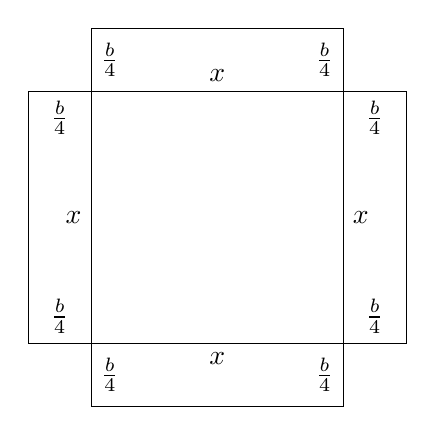
\begin{tikzpicture}[scale=.8]
\coordinate (A) at (0,0);
\coordinate (B) at (4,0);
\coordinate (C) at (4,4);
\coordinate (D) at (0,4);
\draw (A) -- node[below] {$x$} (B) -- node[right] {$x$} (C) -- node[above] {$x$} (D) -- node[left] {$x$} cycle;
\draw (A) -- node[right] {$\frac{b}{4}$} ++(0,-1) -- ++(4,0) -- node[left] {$\frac{b}{4}$} ++(0,1);
\draw (B) -- node[above] {$\frac{b}{4}$} ++(1,0) -- ++(0,4) -- node[below] {$\frac{b}{4}$} ++(-1,0);
\draw (C) -- node[left] {$\frac{b}{4}$} ++(0,1) -- ++(-4,0) -- node[right] {$\frac{b}{4}$} ++(0,-1);
\draw (D) -- node[below] {$\frac{b}{4}$} ++(-1,0) -- ++(0,-4) -- node[above] {$\frac{b}{4}$} ++(1,0);
\end{tikzpicture}
\caption{\R{השטח הוא}\\
=$x^2+4(b/4)x$\\$x^2+bx$}\label{f.khw-1}
\end{subfigure}
\hspace{3em}
\begin{subfigure}[b]{.4\textwidth}
\begin{tikzpicture}[scale=.8]
\coordinate (A) at (0,0);
\coordinate (B) at (4,0);
\coordinate (C) at (4,4);
\coordinate (D) at (0,4);
\draw (A) -- node[below] {$x$} (B) -- node[right] {$x$} (C) -- node[above] {$x$} (D) -- node[left] {$x$} cycle;
\draw (A) -- node[right] {$\frac{b}{4}$} ++(0,-1) -- ++(4,0) -- node[left] {$\frac{b}{4}$} ++(0,1);
\draw (B) -- node[above] {$\frac{b}{4}$} ++(1,0) -- ++(0,4) -- node[below] {$\frac{b}{4}$} ++(-1,0);
\draw (C) -- node[left] {$\frac{b}{4}$} ++(0,1) -- ++(-4,0) -- node[right] {$\frac{b}{4}$} ++(0,-1);
\draw (D) -- node[below] {$\frac{b}{4}$} ++(-1,0) -- ++(0,-4) -- node[above] {$\frac{b}{4}$} ++(1,0);
\draw[thick,dashed] ($(A)+(0,-1)$) -- ++(-1,0) -- ++(0,1);
\draw[thick,dashed] ($(B)+(0,-1)$) -- ++(1,0) -- ++(0,1);
\draw[thick,dashed] ($(C)+(0,1)$) -- ++(1,0) -- ++(0,-1);
\draw[thick,dashed] ($(D)+(0,1)$) -- ++(-1,0) -- ++(0,-1);
\end{tikzpicture}
\caption{\R{השטח הוא}\\
=$x^2+4(b/4)x+4(b/4)^2$\\$x^2+bx+(b^2/4)$}\label{f.khw-2}
\end{subfigure}
\end{center}
\end{figure}
לא ניתן בנות את התרשים ב%
\ref{f.khw-1}
כי אנחנו לא יודעים את ערכו של
$x$,
אבל השטח של הריבוע הגדול ב%
\ref{f.khw-2}
הוא:
\[
x^2+bx+\frac{b^2}{4}=c+\frac{b^2}{4}\,,
\]
שאנחנו כן יודעים כי המקדמים 
$b,c$
נתונים. על ידי בניית התרשים ומחיקת הריבועים הקטנים שצלעותיהם 
$(b/4)$,
עוד ערך ידוע, נקבל קטע קו אורך
$x$.
\begin{example}
נתון
$x^2+12x=64$
אזי
$c+(b^2/4)=64+36=100$
וקל לבנות ריבוע בשטח 
$100$
כי אורכו של כל צלע הוא
$10$.
נחסיר 
$(b/4)+(b/4)=6$,
אורכם של הצלעות של הריבועים הקטנים ונקבל
$x=10-6=4$.
\end{example}

%%%%%%%%%%%%%%%%%%%%%%%%%%%%%%%%%%%%%%%%%%%%%%%%%%%%%%%

\section{הבנייה של
\L{Cardano}
לפתרון משוואה קובית}
\label{s.cardano}

הנוסחה לשורשים של משוואה קובית פורסמה לראשונה במאה ה-%
$16$
על ידי 
\L{Gerolamo Cardano}.
לא נפתח כאן את הנוסחה אבל הרעיון הבסיסי מעניין כי הוא מבוסס על בנייה גיאומטרית בדומה לבנייה של 
\L{al-Khwarizmi}.
הבנייה מתקבלת בצורה פשוטה מאלגברה על ידי פעולת הכפל:
\begin{equation}\label{eq.car}
(a+b)^3=a^3+3a^2b+3ab^2+b^3=(a^3+b^3)+3ab(a+b)\,.
\end{equation}
בגיאומטריה נתחיל עם קוביה שצלעה 
$a+b$
כך שהנפח הוא
$(a+b)^3$.
נפרק את הקוביה לחמישה חלקים. שניים הראשונים הם קוביות שצלעיהן הם
$a$
ו-%
$b$
עם נפח
$a^3$ (כחול)
ו-%
$b^3$ (אדום),
בהתאמה (איור%
~\ref{f.cardano1}).

שלושת החלקים באחרים הם קופסאות (המונח הפורמלי הוא
\L{cuboid}),
כל אחת עם צלע באורך
$a+b$
המתאים לצלע של הקוביה, צלע אחד באורך
$a$
וצלע אחד באורך
$b$,
כך שהנפח של כל שלושת הקופסאות הוא
$ab(a+b)$.
באיור%
~\ref{f.cardano2},
קופסה אחת נמצאת בצד השמאלי של הקוביה (כחול), אחת מאחורי הקוביה (אדום) ואחת מעל לקוביה (ירוק). על ידי צירוף כל חמשת הגופים באיור%
~\ref{f.cardano1}
ובאיור%
~\ref{f.cardano2}
נקבל את משוואה
~\ref{eq.car}.

\begin{figure}[htb]
\begin{center}
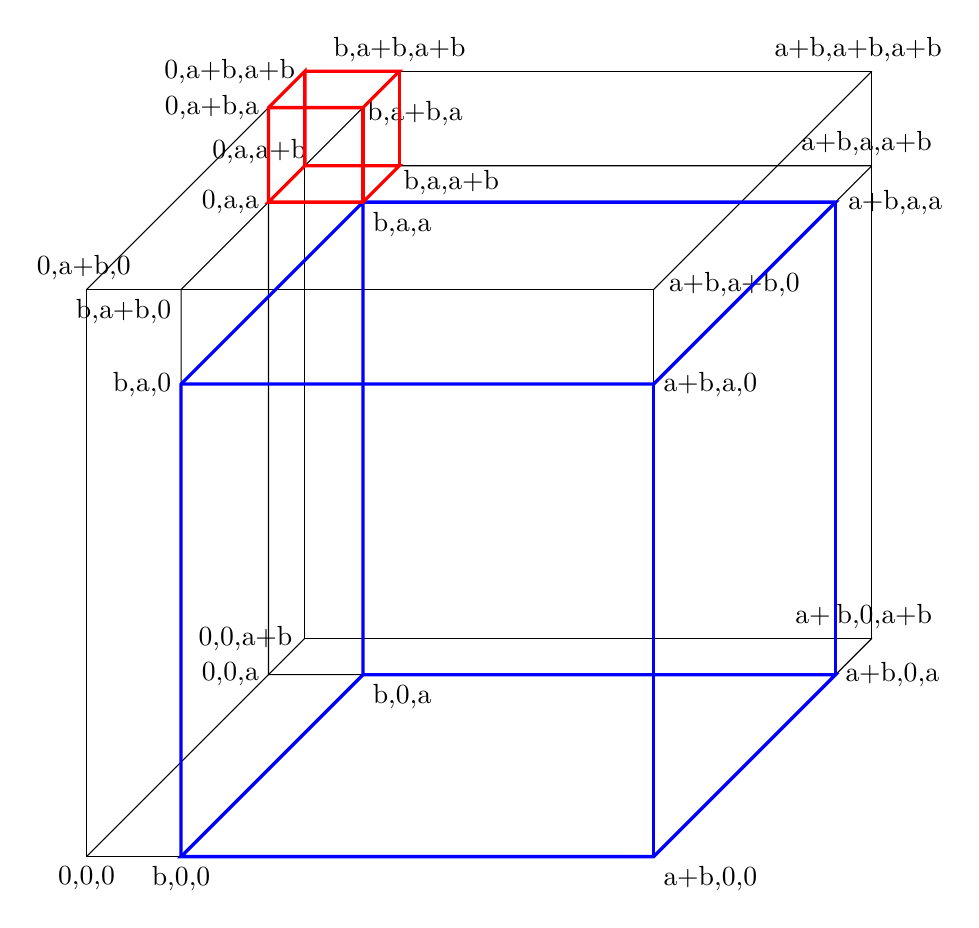
\begin{tikzpicture}[scale=1.2]

% Front face
\coordinate (A) at (0,0,0);
\node[below] at (A) {\sm{0,0,0}};
\coordinate (B) at (6,0,0);
\node[below right] at (B) {\sm{a+b,0,0}};
\coordinate (C) at (6,6,0);
\node[above right,xshift=2pt,yshift=-6pt] at (C)
  {\sm{a+b,a+b,0}};
\coordinate (D) at (0,6,0);
\node[above,xshift=-1pt] at (D) {\sm{0,a+b,0}};

% Front face
\coordinate (FF1) at (1,0,0);
\node[below] at (FF1) {\sm{b,0,0}};
\coordinate (FF2) at (1,5,0);
\node[left] at (FF2) {\sm{b,a,0}};
\coordinate (FF3) at (1,6,0);
\node[below left] at (FF3) {\sm{b,a+b,0}};
\coordinate (FF4) at (6,5,0);
\node[right] at (FF4) {\sm{a+b,a,0}};

% Back face
\coordinate (A1) at (0,0,-6);
\node[left,xshift=-1pt] at (A1) {\sm{0,0,a+b}};
\coordinate (B1) at (6,0,-6);
\node[above,xshift=-3pt] at (B1) {\sm{a+\:b,0,a+b}};
\coordinate (C1) at (6,6,-6);
\node[above,xshift=-5pt] at (C1) {\sm{a+b,a+b,a+b}};
\coordinate (D1) at (0,6,-6);
\node[left] at (D1) {\sm{0,a+b,a+b}};

% Back face
\coordinate (BF1) at (0,5,-6);
\node[above left,xshift=4pt,yshift=-3pt] at (BF1) 
  {\sm{0,a,a+b}};
\coordinate (BF2) at (1,5,-6);
\node[below right,xshift=-2pt,yshift=2pt] at (BF2)
  {\sm{b,a,a+b}};
\coordinate (BF3) at (1,6,-6);
\node[above] at (BF3) {\sm{b,a+b,a+b}};
\coordinate (BF4) at (6,5,-6);
\node[above,xshift=-2pt] at (BF4) {\sm{a+b,a,a+b}};

% Right face
\coordinate (RF1) at (6,5,-5);
\node[right,xshift=1pt] at (RF1) {\sm{a+b,a,a}};
\coordinate (RF2) at (6,0,-5);
\node[right] at (RF2) {\sm{a+b,0,a}};

% Bottom face
\coordinate (BT1) at (1,0,-5);
\node[below right] at (BT1) {\sm{b,0,a}};

% Left face
\coordinate (LF1) at (0,0,-5);
\node[left] at (LF1) {\sm{0,0,a}};
\coordinate (LF2) at (0,5,-5);
\node[left] at (LF2) {\sm{0,a,a}};
\coordinate (LF3) at (0,6,-5);
\node[left] at (LF3) {\sm{0,a+b,a}};

% Top face
\coordinate (TF1) at (1,6,-5);
\node[right,xshift=-2pt,yshift=-2pt] at (TF1) {\sm{b,a+b,a}};

% Internal point
\coordinate (I) at (1,5,-5);
\node[below right] at (I) {\sm{b,a,a}};


\draw (A) -- (B) -- (C) -- (D) -- cycle;
\draw (A1) -- (B1) -- (C1) -- (D1) -- cycle;
\draw (A) -- (A1);
\draw (B) -- (B1);
\draw (C) -- (C1);
\draw (D) -- (D1);

\draw (FF1) -- (FF2) -- (FF3) -- (BF3);
\draw (BF2) -- (FF2) -- (FF4) -- (BF4);
\draw (FF1) -- (BT1) -- (TF1);
\draw (BF3) -- (BF2);
\draw (TF1) -- (LF3);
\draw (LF3) -- (LF1) -- (RF2) -- (RF1) -- (LF2) -- 
      (BF1) -- (BF4);

\draw[very thick,blue] (FF1) -- (B) -- (RF2) -- (BT1) -- cycle; 
\draw[very thick,blue] (FF1) -- (FF2) -- (I) -- (BT1);
\draw[very thick,blue] (I) -- (RF1) -- (FF4) -- (FF2);
\draw[very thick,blue] (FF4) -- (B);
\draw[very thick,blue] (RF1) -- (RF2);

\draw[very thick,red] (I) -- (LF2) -- (BF1) -- (BF2) -- cycle;
\draw[very thick,red] (LF2) -- (LF3) -- (D1) -- (BF1);
\draw[very thick,red] (D1) -- (BF3) -- (TF1) -- (LF3);
\draw[very thick,red] (TF1) -- (I);
\draw[very thick,red] (BF3) -- (BF2);

\end{tikzpicture}
\end{center}
\caption{$(a^3+b^3)=(a^3+b^3)+\cdots$}\label{f.cardano1}
\end{figure}

%%%%%%%%%%%%%%%%%%%%%%%%%%%%%%%%%%%%%%%%%%%%%%%%%%%%%%%%%%%%%

\begin{figure}[htb]
\begin{center}
\begin{tikzpicture}[scale=1.2]

% Front face
\coordinate (A) at (0,0,0);
\node[below] at (A) {\sm{0,0,0}};
\coordinate (B) at (6,0,0);
\node[below right] at (B) {\sm{a+b,0,0}};
\coordinate (C) at (6,6,0);
\node[above right,xshift=2pt,yshift=-6pt] at (C)
  {\sm{a+b,a+b,0}};
\coordinate (D) at (0,6,0);
\node[above,xshift=-1pt] at (D) {\sm{0,a+b,0}};

% Front face
\coordinate (FF1) at (1,0,0);
\node[below] at (FF1) {\sm{b,0,0}};
\coordinate (FF2) at (1,5,0);
\node[left] at (FF2) {\sm{b,a,0}};
\coordinate (FF3) at (1,6,0);
\node[below left] at (FF3) {\sm{b,a+b,0}};
\coordinate (FF4) at (6,5,0);
\node[right] at (FF4) {\sm{a+b,a,0}};

% Back face
\coordinate (A1) at (0,0,-6);
\node[left,xshift=-1pt] at (A1) {\sm{0,0,a+b}};
\coordinate (B1) at (6,0,-6);
\node[above,xshift=-3pt] at (B1) {\sm{a+\:b,0,a+b}};
\coordinate (C1) at (6,6,-6);
\node[above,xshift=-5pt] at (C1) {\sm{a+b,a+b,a+b}};
\coordinate (D1) at (0,6,-6);
\node[left] at (D1) {\sm{0,a+b,a+b}};

% Back face
\coordinate (BF1) at (0,5,-6);
\node[above left,xshift=4pt,yshift=-3pt] at (BF1) 
  {\sm{0,a,a+b}};
\coordinate (BF2) at (1,5,-6);
\node[below right,xshift=-2pt,yshift=2pt] at (BF2)
  {\sm{b,a,a+b}};
\coordinate (BF3) at (1,6,-6);
\node[above] at (BF3) {\sm{b,a+b,a+b}};
\coordinate (BF4) at (6,5,-6);
\node[above,xshift=-2pt] at (BF4) {\sm{a+b,a,a+b}};

% Right face
\coordinate (RF1) at (6,5,-5);
\node[right,xshift=1pt] at (RF1) {\sm{a+b,a,a}};
\coordinate (RF2) at (6,0,-5);
\node[right] at (RF2) {\sm{a+b,0,a}};

% Bottom face
\coordinate (BT1) at (1,0,-5);
\node[below right] at (BT1) {\sm{b,0,a}};

% Left face
\coordinate (LF1) at (0,0,-5);
\node[left] at (LF1) {\sm{0,0,a}};
\coordinate (LF2) at (0,5,-5);
\node[left] at (LF2) {\sm{0,a,a}};
\coordinate (LF3) at (0,6,-5);
\node[left] at (LF3) {\sm{0,a+b,a}};

% Top face
\coordinate (TF1) at (1,6,-5);
\node[right,xshift=-2pt,yshift=-2pt] at (TF1) {\sm{b,a+b,a}};

% Internal point
\coordinate (I) at (1,5,-5);
\node[below right] at (I) {\sm{b,a,a}};


\draw (A) -- (B) -- (C) -- (D) -- cycle;
\draw (A1) -- (B1) -- (C1) -- (D1) -- cycle;
\draw (A) -- (A1);
\draw (B) -- (B1);
\draw (C) -- (C1);
\draw (D) -- (D1);

\draw (FF1) -- (FF2) -- (FF3) -- (BF3);
\draw (BF2) -- (FF2) -- (FF4) -- (BF4);
\draw (FF1) -- (BT1) -- (TF1);
\draw (BF3) -- (BF2);
\draw (TF1) -- (LF3);
\draw (LF3) -- (LF1) -- (RF2) -- (RF1) -- (LF2) -- 
      (BF1) -- (BF4);

\draw[very thick,blue] (A) -- (FF1) -- (FF3) -- (D) -- cycle;
\draw[very thick,blue] (FF1) -- (BT1) -- (TF1) -- (FF3);
\draw[very thick,blue] (TF1) -- (LF3) -- (D);
\draw[very thick,blue] (LF3) -- (LF1) -- (A);
\draw[very thick,blue] (LF1) -- (BT1);

\draw[very thick,red] (LF1) -- (RF2) -- (RF1) -- (LF2);
\draw[very thick,red] ($(LF2) + (2pt,0)$) -- ($(LF1) + (2pt,0)$);
\draw[very thick,red] (A1) -- (B1) -- (BF4) -- (BF1) -- cycle;
\draw[very thick,red] ($(LF2) + (2pt,0)$) -- ($(BF1) + (2pt,0)$);
\draw[very thick,red] (BF4) -- (RF1);
\draw[very thick,red] (B1) -- (RF2);
\draw[very thick,red] (A1) -- (LF1);

\draw[very thick,green] (FF2) -- (FF4) -- (C) -- (FF3);
\draw[very thick,green] 
  ($(FF2) + (2pt,0)$) -- ($(FF3) + (2pt,0)$);
\draw[very thick,green] 
  ($(FF4) + (0,2pt)$) -- ($(BF4) + (0,2pt)$);
\draw[very thick,green] (BF4) -- (C1) -- (BF3);
\draw[very thick,green] 
  ($(BF3) + (2pt,0)$) -- ($(FF3) + (2pt,0)$);
\draw[very thick,green] (C1) -- (C);
\draw[very thick,green] (BF3) -- (BF2) -- (FF2);
\draw[very thick,green] 
  ($(BF2) + (0,2pt)$) -- ($(BF4) + (0,2pt)$);


\end{tikzpicture}
\end{center}
\caption{$(a^3+b^3)=\cdots+3ab(a+b)$}\label{f.cardano2}
\end{figure}

%%%%%%%%%%%%%%%%%%%%%%%%%%%%%%%%%%%%%%%%%%%%%%%%%%%%%%%

\section{הם לא נרתעו ממספרים דמיוניים}\label{s.imaginary}

ההיסטוריה של המתמטיקה מתאפיינת בסדרה של מושגים שתחילה נחשבו כחסרי משמעות, אבל לבסוף הובנו, התקבלו והוכיחו את חשיבותם. "ברור" ש-%
$-1$,
מספר שלילי, חסר משמעות כי מספרים סופרים דברים. "ברור" ש-%
$\sqrt{2}$,
מספר לא רציונלי, חסר משמעות כי מספר הוא יחס בין שני מספרים שלמים. "ברור" ש-%
$\sqrt{-1}$, 
השורש של מספר שלילי, חסר משמעות כי אין מספר שהריבוע שלו שלילי.

הבנה של השורשים של מספרים שליליים, שעד היום קוראים להם מספרים 
\textbf{דמיוניים}
\L{\textbf{\small (imaginary)}}
למרות שהם לא פחות ממשיים ממספרים ממשיים, לא הושגה עד המאה התשע עשרה. לכן, מפתיע שכבר במאה השש עשרה,
\L{Geralamo Cardano}
ו-%
\L{Rafael Bombelli}
סירבו להירתע מהמושג וצעדו את הצעדים הראשונים הקטנים לקראת הבנה המספרים הללו.

נוכל להשתמש בנוסחה הרגילה 
(משוואה%
~\ref{eq.quadratic-roots})
עבור המשוואה הריבועית:
\begin{equation}
x^2-10x+40=0\,,\label{eq.cardano-quadratic}
\end{equation}
ונקבל:
\[
r_1, r_2=\displaystyle\frac{10\pm\sqrt{100-160}}{2}=5\pm\sqrt{-15}\,.
\]
אמנם אין אנו יודעים מהם השורשים של מספרים שליליים ולא את ערכם, אבל כמו
\L{Cardano}
אנו יודעים שלפי משפט%
~\ref{thm.roots-coefficients}
ש:
\begin{eqn}
r_1+r_2&=&(5+\sqrt{-15})+(5-\sqrt{-15})=10=-b\\
r_1r_2&=&(5+\sqrt{-15})(5-\sqrt{-15})=\\
&=&25-\sqrt{-15}\cdot\sqrt{-15}=25-(-15)=40=c\,.
\end{eqn}
שהן המקדמים של המשוואה הריבועית
~\ref{eq.cardano-quadratic}.
די אינטואיטיבית ש-%
$\sqrt{-15}+(-\sqrt{-15})=0$
גם אם אין אנו יודעים כלום על
$\sqrt{-15}$,
ודי אינטואיטיבית ש-%
$\sqrt{-15}\cdot-(\sqrt{-15})=-(-15)=15$
גם אם אין אנו יודעים כלום על
$\sqrt{-15}$.

נעיין במשוואה הקובית:
\begin{equation}
x^3-15x-4=0\,.\label{eq.bombelli-cubic}
\end{equation}
לא קשה למצוא ש-%
$4$
הוא שורש, אבל איך אפשר לחשב אותו? לפי הנוסחה של
\L{Cardano}
השורש הוא:
\begin{equation}
r=\sqrt[3]{2+11\sqrt{-1}}+\sqrt[3]{2-11\sqrt{-1}}\,,\label{eq.cube-root}
\end{equation}
אבל זאת נוסחה די סבוכה שלא נראה שיש קשר בינה לבין
$4$. 

\L{Bombelli}
גילה אומץ לב וחישוב את החישוב שלהן (ראו משוואה%
~\ref{eq.car}):
\begin{eqn}
(2+\sqrt{-1})^3&=&
8+3\cdot 4\sqrt{-1}+3\cdot 2(-1)+(-1\sqrt{-1})=
2+11\sqrt{-1}\\
(2-\sqrt{-1})^3&=&
8-3\cdot 4\sqrt{-1}+3\cdot 2(-1)-(-1\sqrt{-1})=
2-11\sqrt{-1}\,.
\end{eqn}
לפי משוואה%
~\ref{eq.cube-root}:
\begin{eqn}
r&=&\sqrt[3]{2+11\sqrt{-1}} + \sqrt[3]{2-11\sqrt{-1}}\\
&=&\sqrt[3]{(2+\sqrt{-1})^3} + \sqrt[3]{(2-\sqrt{-1})^3}\\
&=&(2+\sqrt{-1}) + (2-\sqrt{-1})=4\,.
\end{eqn}


%%%%%%%%%%%%%%%%%%%%%%%%%%%%%%%%%%%%%%%%%%%%%%%%%%%%%%%%

\section{השיטה של 
\L{Lill}
והמעגל של
\L{Carlyle}}\label{s.lill-quadratic}

ניתן להשתמש בשיטה של
\L{Lill}
כדי לפתור משוואות ריבועיות.%
\footnote{סעיף זה מניח שקראתם על השיטה של
\L{Lill}
בפרק%
~\ref{c.origami-cube}.}
נדגים את השיטה על משוואה%
~\ref{eq.quadratic-lill}
ששורשיה מתקבלות על ידי פירוק לגורמים:
\[
x^2+bx+c=x^2-4x+3= (x-1)(x-3)\,.
\]
מהשיטה של
\L{Lill}
נקבל את המסלולים באיור%
~\ref{f.lill-quadratic}.

\begin{figure}[hbt]
\begin{center}
\begin{tikzpicture}[scale=1.1]
% Draw help lines and axes
\draw[step=10mm,white!50!black] (-4,-5) grid (2,1);
\draw[thick] (-4,0) -- (2,0);
\draw[thick] (0,-5) -- (0,1);
\foreach \x in {-3,...,2}
  \node at (\x-.2,.2) {\sm{\x}};
\foreach \y in {-4,...,-1}
  \node at (-.2,\y-.3) {\sm{\y}};

 Draw first path
\coordinate (A) at (0,0);
\coordinate (B) at (1,0);
\coordinate (C) at (1,-4);
\coordinate (D) at (-2,-4);
\draw[very thick] (A) --
  node[above] {$1$} (B);
\draw[very thick,name path=bc] (B) -- 
  node[right,xshift=-1pt,yshift=6pt] {$b=-4$} (C);
\draw[very thick,name path=cd] (C) --
  node[below left,xshift=3pt] {$c=3$}(D);

% Draw first segment of second path
\path[name path=a2] (A) -- +(-45:1.414);
\path [name intersections = {of = a2 and bc, by = {A2}}];
\node[above right] at (A2) {$P_1$};
\draw[very thick,dashed] (A) -- (A2);
\draw ($(A) + (14pt,0)$)
  arc [start angle=0, end angle = -45, radius=14pt];
\node[below right,xshift=40pt,yshift=-2pt] at (A) {$-45^\circ$};
\draw[->] ($(A)+(33pt,-6pt)$) -- +(-18pt,0);
\draw[rotate=135] (A2) rectangle +(5pt,5pt);

% Draw second segment of second path
\path[name path=b2] (A2) -- +(-135:5);
\path [name intersections = {of = b2 and cd, by = {B2}}];
\draw[very thick,dashed] (A2) -- (B2);

% Draw first segment of second path
\path[name path=a3] (A) -- +(-71.57:4);
\path [name intersections = {of = a3 and bc, by = {A3}}];
\node[above right] at (A3) {$P_2$};
\draw[very thick,dashed] (A) -- (A3);
\draw ($(A) + (20pt,0)$)
  arc [start angle=0, end angle = -71.57, radius=20pt];
\node[below right,xshift=40pt,yshift=-10pt] at (A) {$-71.57^\circ$};
\draw[->] ($(A)+(35pt,-13pt)$) -- +(-18pt,0);
\draw[rotate=108.43] (A3) rectangle +(5pt,5pt);

% Draw second segment of second path
\path[name path=b3] (A3) -- +(198.43:5);
\path [name intersections = {of = b3 and cd, by = {B3}}];
\draw[very thick,dashed] (A3) -- (B3);

\end{tikzpicture}
\end{center}
\caption{השיטה של
\L{Lill}
עבור
$x^2-4x+3$}\label{f.lill-quadratic}
\end{figure}
נבדוק שהזוויות נכונות:
\[
-\tan (-45^\circ) = -1,\quad -\tan (-71.57^\circ) \approx -3\,.
\]
עבור משוואות ריבועיות ניתן למצוא
$P_1,P_2$
שהן נקודות החיתוך של הקו המייצג את המקדם
$b$
והמעגל שקוטרו הוא הקו המחבר את נקודת ההתחלה ונקודת הסיום של המסלולים (איור%
~\ref{f.lill-circle}).
כדי שנקודה על הקו
$b$
תהיה שורש, השיקוף של הקו בצריך להיות 
$90^\circ$ 
ולכן הזווית כלואה על ידי קוטר.
\begin{figure}[htb]
\begin{center}
\begin{tikzpicture}[scale=1]
% Draw help lines and axes
\draw[step=10mm,white!50!black] (-4,-5) grid (2,1);
\draw[thick] (-4,0) -- (2,0);
\draw[thick] (0,-5) -- (0,1);
\foreach \x in {-3,...,2}
  \node at (\x-.2,.2) {\sm{\x}};
\foreach \y in {-4,...,-1}
  \node at (-.2,\y-.3) {\sm{\y}};

 Draw first path
\coordinate (A) at (0,0);
\coordinate (B) at (1,0);
\coordinate (C) at (1,-4);
\coordinate (D) at (-2,-4);
\draw[very thick] (A) --
  node[above] {$1$} (B);
\draw[very thick,name path=bc] (B) -- 
  node[right,xshift=-2pt,yshift=6pt] {$b=-4$} (C);
\draw[very thick,name path=cd] (C) --
  node[below left,xshift=-1pt,yshift=-5pt] {$c=3$}(D);

% Draw first segment of second path
\path[name path=a2] (A) -- +(-45:1.414);
\path [name intersections = {of = a2 and bc, by = {A2}}];
\node[above right] at (A2) {$P_1$};
\draw[dashed] (A) -- (A2);
\draw ($(A) + (14pt,0)$)
  arc [start angle=0, end angle = -45, radius=14pt];
\node[below right,xshift=40pt,yshift=-2pt] at (A) {$-45^\circ$};
\draw[->] ($(A)+(33pt,-6pt)$) -- +(-18pt,0);
\draw[rotate=135] (A2) rectangle +(5pt,5pt);

% Draw second segment of second path
\path[name path=b2] (A2) -- +(-135:5);
\path [name intersections = {of = b2 and cd, by = {B2}}];
\draw[dashed] (A2) -- (B2);

% Draw first segment of second path
\path[name path=a3] (A) -- +(-71.57:4);
\path [name intersections = {of = a3 and bc, by = {A3}}];
\node[above right] at (A3) {$P_2$};
\draw[dashed] (A) -- (A3);
\draw ($(A) + (20pt,0)$)
  arc [start angle=0, end angle = -71.57, radius=20pt];
\node[below right,xshift=40pt,yshift=-10pt] at (A) {$-71.57^\circ$};
\draw[->] ($(A)+(35pt,-13pt)$) -- +(-18pt,0);
\draw[rotate=108.43] (A3) rectangle +(5pt,5pt);

% Draw second segment of second path
\path[name path=b3] (A3) -- +(198.43:5);
\path [name intersections = {of = b3 and cd, by = {B3}}];
\draw[dashed] (A3) -- (B3);

\coordinate (O) at (-1,-2);
\vertex{O};
\node[draw,circle through=(A)] at (O) {};
\draw[very thick,dotted] (A) -- (D);

\end{tikzpicture}
\end{center}
\caption{בניית מעגל כדי למצוא את השורשים}\label{f.lill-circle}
\end{figure}
ניתן לבדוק באמצעות חישוב. מרכז המעגל הוא $(-1,-2)$, נקודת האמצע של הקוטר. אורך הקוטר הוא:
\[
\sqrt{(-2)^2+(-4)^2}=\sqrt{20}\,,
\]
ולכן הריבוע של הרדיוס הוא
$\left(\sqrt{20/2}\right)^2=5$. 
אנו מחפשים את החיתוך של מעגל זה עם הקו
$x=1$:
\begin{eqn}
(x-(-1))^2+(y-(-2))^2&=&r^2\\
(x^2+2x+1)+(y^2+4y+4)&=&5\\
y^2+4y+3&=&0\\
y&=&-1,\;-3\,.
\end{eqn}
שיטה דומה לפתרון של משוואות ריבועיות היא מעגלי
\L{Carlyle}
שקודמת לשיטה של
\L{Lill}.
ניתן משוואה ריבועית
$x^2-bx+c$
(שימו לב שסימן המינוס בגורם הליניארי), נבנה נקודות
$(0,1)$
ו-%
$(b,c)$
ומעגל שקוטרו הוא הקו המחבר את שתי הנקודות (איור%
~\ref{f.carlyle-circle}).
החיתוכים עם ציר ה-%
$x$
(אם הם קיימים) הם השורשים של המשוואה.

במקרה הכללי, מרכז המעגל הוא
$(b/2,(c-(-1))/2)$
ואורך הקוטר הוא
$\sqrt{b^2+(c-1)^2}$,
כך שמשוואות המעגל היא:
\[
\left(x-\frac{b}{2}\right)^2+\left(y-\frac{c+1}{2}\right)^2=
\frac{b^2+(c-1)^2}{4}\,.
\]
למשל, אם נציב
$b=4,c=,y=0$, 
נראה ש-%
$x=1,x=3$
הם השורשים של המשוואה הריבועית.
\begin{figure}[htb]
\begin{center}
\begin{tikzpicture}[scale=1]
% Draw help lines and axes
\draw[step=10mm,white!50!black] (-1,-1) grid (5,5);
\draw[thick] (-1,0) -- (5,0);
\draw[thick] (0,-1) -- (0,5);
\foreach \x in {0,...,5}
  \node at (\x-.2,.2) {\sm{\x}};
\foreach \y in {1,...,4}
  \node at (-.1,\y+.2) {\sm{\y}};

\coordinate (A) at (0,1);
\node[below left] at (A) {$(0,1)$};
\coordinate (B) at (4,3);
\node[above right] at (B) {$(4,3)$};
\vertex{A};
\vertex{B};

\coordinate (O) at (2,2);
\vertex{O};
\node[draw,circle through=(B)] at (O) {};
\draw[very thick,dotted] (A) -- (B);

\coordinate (X1) at (1,0);
\node[below left] at (X1) {$(1,0)$};
\coordinate (X2) at (3,0);
\node[below right] at (X2) {$(3,0)$};
\vertex{X1};
\vertex{X2};

\end{tikzpicture}
\end{center}
\caption{השיטה של
\L{Carlyle}
עבור
$x^2-4x+3$}\label{f.carlyle-circle}
\end{figure}

%%%%%%%%%%%%%%%%%%%%%%%%%%%%%%%%%%%%%%%%%%%%%%%%%%%%%%%

\section{חישוב נומרי של שורשים}\label{s.numerical}

סטודנטים לומדים חישוב סימבולי של שורשים, נגזרות, וכו'. היום, רוב החישובים מתבצעים על ידי מחשבים, כך שחישוב סימבולי פחות חשוב. 
\textbf{אנליזה נומרית}
היא תחום במתמטיקה ומדעי המישב בו מפתחים שיטות חישוב מדוייקות ויעילות. האתגר המרכזי היא לטפל בסופיות של ערכים שנשמרים בזיכרון של המחשב. קל לבצע את החישוב:
\[0.12\times 0.14=0.0168\]
אבל כדי לחשב:
\[0.123456789\times 0.123456789\]
המחשב חייב לשמור שמונה עשרה ספרות דרישה שאי-אפשר למלא כאשר לתאי הזיכרון במחשב מסוגל לשמור שש עשרה ספרות בלבד. שגיאה זו נקראת 
\textbf{שגיאת עיגול \L{(round-off error)}}.

בעיה חמורה יותר מופיעה כאשר החישובים מבוצעים ב-%
\textbf{נקודה צפה \L{\small floating point}}.
ברור שלא נחשב את
\[(0.12\times 10^{-10})\times (0.14\times 10^{-8})\]
על ידי רישום כל ספרות האפס. במקום זה, נכפיל את המנטיסות [???]
\L{\small (mantissas)}
ונחבר את המעריכים [???] 
\L{\small (exponents)}
כדי לקבל
$0.0168\times 10^{-18}$
שעוברת נירמול ל-%
$0.168\times 10^{-19}$
כך שהספרה 
\L{\small most significant ????}
תופיע ליד הנקודה העשרונית. זה מאפשר להשתמש במספר הספרות המירבי בהינתן מנטיסה באורך קבוע. אם המעריך הגבוה ביותר שניתן לשמור הוא 
$-16$
פשוט לא ניתן לייצג את המספר בזיכרון. שגיאה זו נקראת 
\textbf{\L{floating-point underflow????}}.

הנוסחה למציאת השורשים של המשוואה הריבועית
$x^2+bx+c$ 
היא:
\begin{equation}
r_1, r_2 = \frac{-b\pm\sqrt{b^2-4c}}{2}\,.\label{eq.quadratic-numerical}
\end{equation}
מה קורה עם
$b=1000$
ו-%
$c=4$.
השורשים הם:
\[
r_1, r_2 = \frac{-1000\pm\sqrt{1000000-16}}{2}\,.
\]
בתלות בדיוק של החישובים, אפשר שאחת השורשים כל כך קרובה לאפס שהערך שנשמר הוא אפס. אם נציב אפס במשוואה נקבל את התוצאה המפתיעה
$0^2+b\cdot 0 +4= 4= 0$.

האם יש שיטה טובה יותר? לפי משוואה%
~\ref{eq.viete-quad}:
\[
r_1+r_2 = -b\,,\quad\quad r_1r_2=c\,.
\]
אם
$r_2$
ממש קטן יותר מ-%
$r_1$,
שנסמן
$r_2\ll r_1$,
אזי
$r_1\approx -b$
ו-%
$r_2=c/b$.
טבלה%
~\ref{t.quadratic},
שחושבה באמצעות תכנית מחשב, משווה את ערכי השורשים המחשבים לפי הנוסחאות הללו אל הערכים המתקבלים מהנוסחה הרגילה, משוואה%
~\ref{eq.quadratic-numerical}.
הערך של
$c$
נקבע ל-%
$4$
והטבלה מראה את השורשים של ערכים הולכים וגדלים של
$b$.

תחילה, הערכים האמיתיים שחושבו באמצעות הנוסחה הרגילה עבור
$r_2$
מדוייקים יותר
($r_2-r_{2v}$ שלילי)
אבל החל מ-%
$b=100000$
החישוב שמבוסס על משוואה%
~\ref{eq.viete-quad}
מדוייקת יותר. כך הן ההפתעות של אנליזה נומרית.


\begin{table}[bht]
\caption[שני חישובים של השורשים של משוואה ריבועית]%
{שני חישובים של השורשים של משוואה ריבועית.
$r_1,r_2$
הם השורשים שחושבו לפי משוואה%
~\ref{eq.quadratic-numerical}.
$r_{1v},r_{2v}$
הם השורשים שחושבו לפי משוואה%
~\ref{eq.viete-quad}.
השגיאות הן
$r_{i}-r_{iv}$.
מספרים בנקודה צפה נכתבו כ-%
$-4e-5$
במקום
$4\times 10^{-5}$
כי תכניות מחשב נכתבים לרוב כסדרה ליניארית של סימנים
.} \label{t.quadratic}
\begin{footnotesize}
\[
\begin{array}{r@{\hspace{2.5mm}}r@{\hspace{2.5mm}}r@{\hspace{2.5mm}}r@{\hspace{2.5mm}}r@{\hspace{2.5mm}}r@{\hspace{2.5mm}}r}
\hline
b & r_1 & r_{1v} & \mathrm{Error}_1 & r_2 & r_{2v} & \mathrm{Error}_2\\
\hline
100  &  -99.9599  &  -100  &  0.0400  &  -0.04001\  &  -0.04  &  -1.6012e\!-\!05\\
1000  &  -999.9959  &  -1000  &  0.0040  &  -0.0040  &  -0.004  &  -1.6000e\!-\!08\\
10000  &  -9999.9996  &  -10000  &  0.0004  &  -0.0004  &  -0.0004  &  -1.6270e\!-\!11\\
100000  &  -99999.9999  &  -100000  &  3.9999e\!-\!5  &  -3.9999e\!-\!5  &  -4e\!-\!5  &  1.0104e\!-\!12\\
1000000  &  -999999.9999  &  -1000000  &  4.0000e\!-\!6  &  -3.9999e\!-\!6  &  -4e\!-\!6  &  2.7749e\!-\!11\\
10000000  &  -10000000.0  &  -10000000  &  3.9860e\!-\!7  &  -3.9953e\!-\!7  &  -4e\!-\!7  &  4.6261e\!-\!10\\
\hline
\end{array}
\]
\end{footnotesize}
\end{table}

\subsection*{מה  ההפתעה?}

השיטה של 
\L{Poh-Shen Loh}
מביא הסתכלות חדשה על היחס בין המקדמים לשורשים שלא רואים כאשר לומדים בעל פה את הנוסחה הרגילה. מה שמפתיע הוא שיחס זה עקרוני בהוכחה האלגברית של 
\L{Gauss}
שניתן לבנות מצולע משוכלל עם שבעה עשר צלעות (פרק%
~\ref{c.heptadecagon}).

עם השליטה המודרנית של שיטות אלגבריות בגיאומטריה, חשוב לזכור שפעם המצב היה הפוך. כפי שרואים מהבניות של
\L{Al-Khwarizmi}
ו-%
\L{Cardano},
השיטות הגיאומטריות שימשו פעם כדי להוכיח תוצאות באלגברה. 
\L{Lill}
ו-%
\L{Carlyle}
פיתחו שיטות גיאומטריות לפתרון של משוואות ריבועיות.
שיקולים של חישובים נומריים יפתיעו סטודנטים שלא נחשפו קודם לנושא.

\subsection*{מקורות}
השיטה של
\L{Poh-Shen Loh}
פרוסמה ב-%
\cite{loh1,loh2}.
הבנייה של
\L{Al-Khwarizmi}
נמצאת ב-%
\cite[פרק 1]{jorg}
וב-%
\cite{mastin}.
ניתן למצוא את הבנייה של 
\L{Cardano}
ב-%
\cite[פרק 1]{jorg}.
ההיסטוריה הצבעונית של הפיתוח של הנוסחה של
\L{Cardano}
מסופרת ב-%
\cite{wiki:cardano}.
תיאור הניסיונות הראשונים לחישוב על מספרים דמיוניים נלקח מ-%
\cite[פרק 2]{jorg}. 
\cite{wiki:quadratic}
מציג את השיטה של 
\L{Lill}
והמעגל של 
\L{Carlyle}
ביחד עם דיון על חישוב נומרי של השורשים.

